
\section{Experiments}\label{experiments}

\paragraph{Experimental Setup}Replica exchange requires a within chain MCMC algorithm.
For finite dimensional continuous models we use the No U-Turn Sampler \cite{hoffman2014no}, a variant of Hamiltonion Monte Carlo (HMC).
We use reverse-mode automatic differentiation \cite{griewank2008evaluating} to compute the negative log gradient of $f$, which is required for HMC.
For other models we use standard Metropolis Hastings by defining proposals on elements in the dictionary.
In particular we use the single site Metropolis Hastings (SSMH) \cite{wingate2011lightweight} which modifies a single random variable at a time.

Replica exchange has a number of hyper-parameters: the number of parallel chains, the corresponding temperatures, the swapping schedule.
Several good practices are outlined in \cite{earl2005parallel}.  In practice, we logarithmically space $\alpha$ between a lower and upper bound (e.g., $\log_{10}(\alpha_1) = 5$ to $\log_{10}(\alpha_M) = -5$), and swap states of chains that are adjacent in temperature ($\alpha_1$ with $\alpha_2$, $\alpha_2$ with $\alpha_3$, etc) periodically.


\paragraph{Small Models}
In Figure \ref{fig:density} we use conditioning to truncate a normal distribution. Figure  \ref{gridn} shows histograms of samples from a uniform prior  $[-1, 1]^2$ conditioned on a variety of predicates.  While simple, these examples can be challenging due to discontinuities in the approximate posterior.

% \begin{figure}[!htb]
% 	\centering
% 	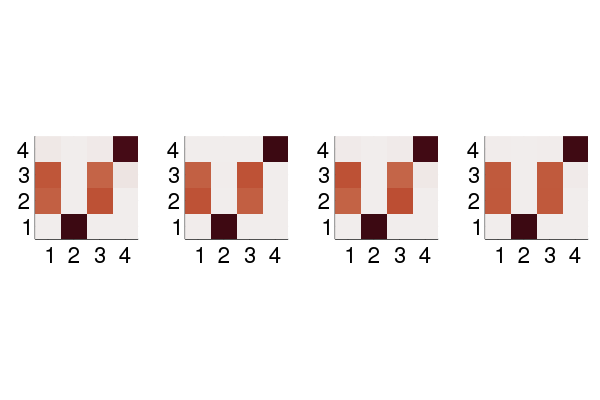
\includegraphics[width=0.9\linewidth]{swapmats}
% 	\caption{Analysis of Replica Exchange}
% 	\label{swapmats}
% \end{figure}	


\begin{figure}[!htb]
	\centering
	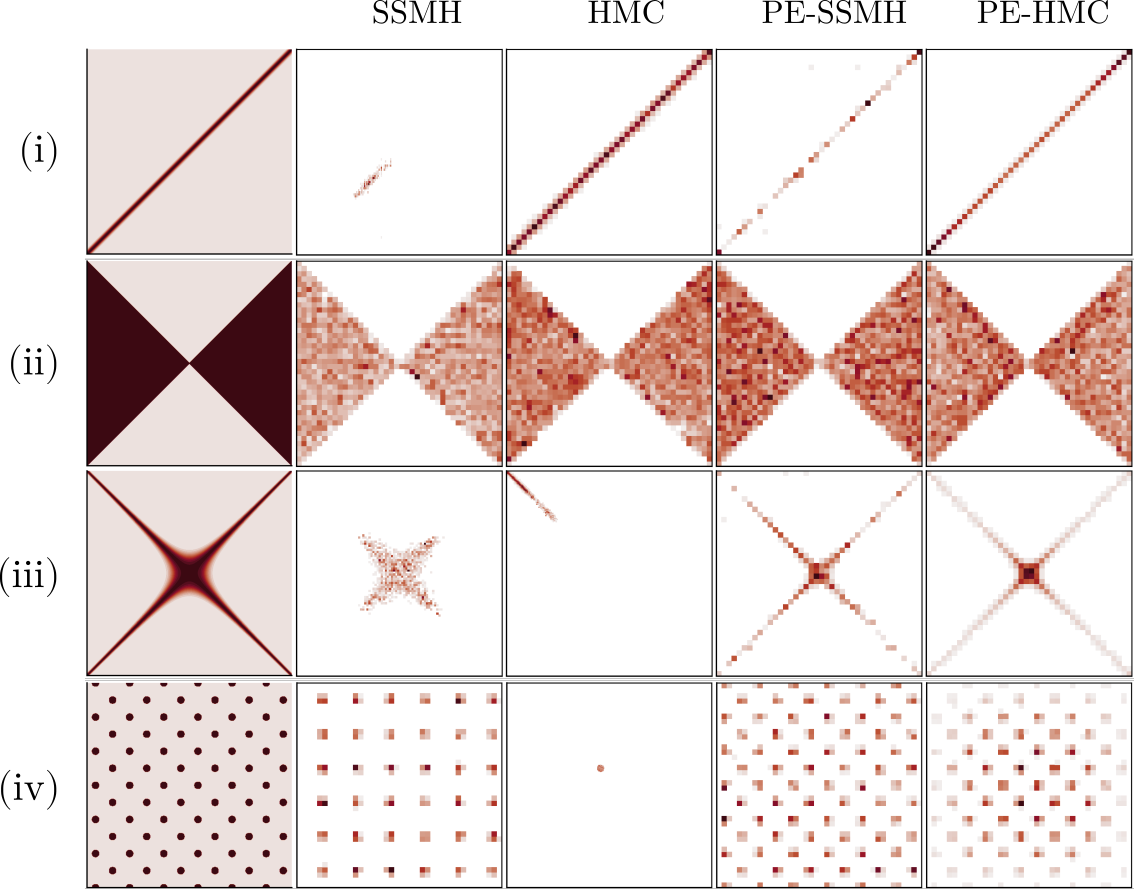
\includegraphics[width=0.9\linewidth]{gx2}
	\caption{Samples from models using different procedures.  Each model is $x,y \sim \unif(-1,1)$ conditioned on (i) $x \soft{=} y$, (ii) $|x| \soft{>} |y|$, (iii) $x^2 \soft{=} y^2$ and (iv) $\sin(kx)\cos(kx) \soft{>} 0.9999$.
	Inference procedures are: Single Site Metropolis Hastings (SSMH), Hamiltonian Monte Carlo (HMC), and Predicate-Exchange (PE) using HMC and SSMH within chain.}
	\label{gridn}
\end{figure}	

\begin{figure}[!htb]
\centering
\textbf{Truncated Normal through Conditioning}\par\medskip
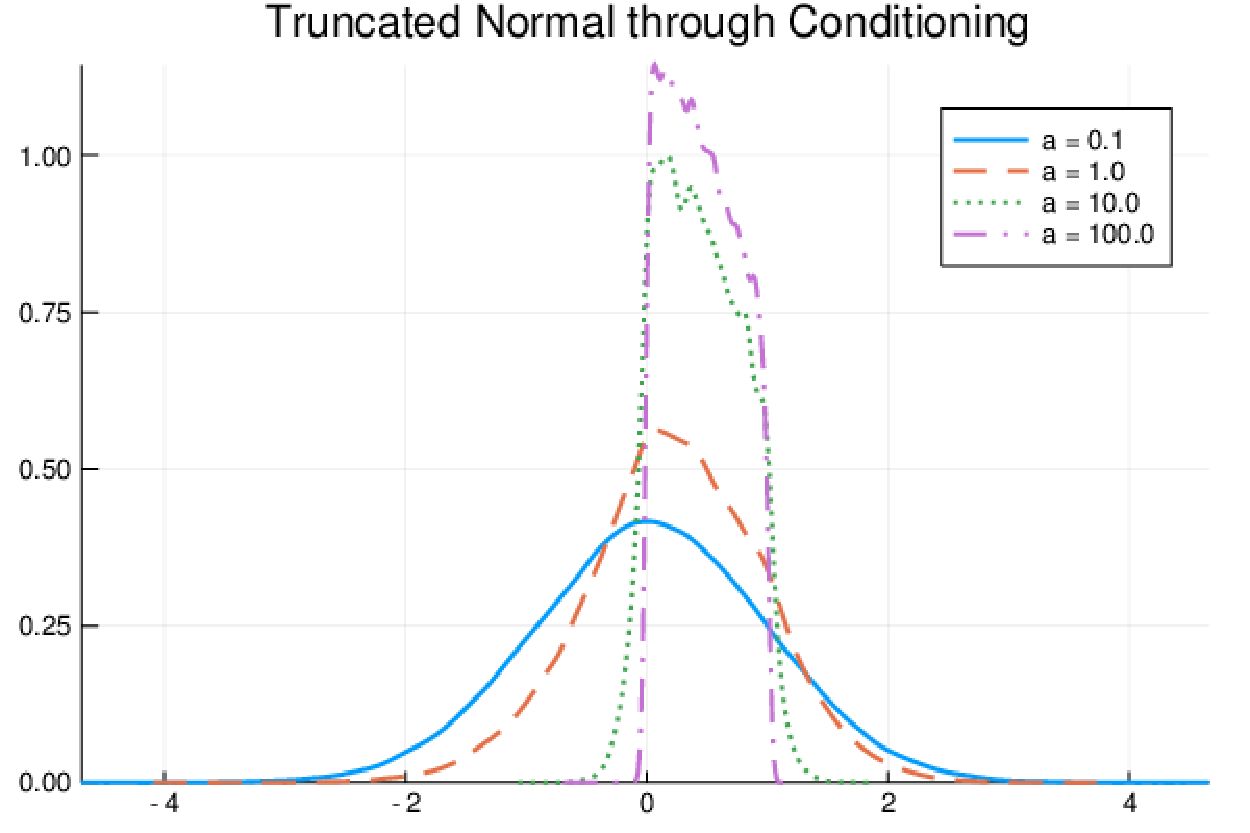
\includegraphics[width=0.55\linewidth,trim={0.5cm, .3cm, .5cm, .1cm}, clip]{truncated}
% \fbox{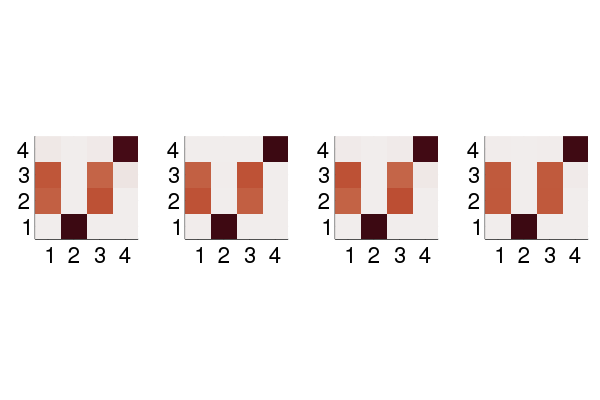
\includegraphics[width=0.40\linewidth,trim={2.0cm, .2cm, 2cm, 1.2cm}, clip]{swapmats}}
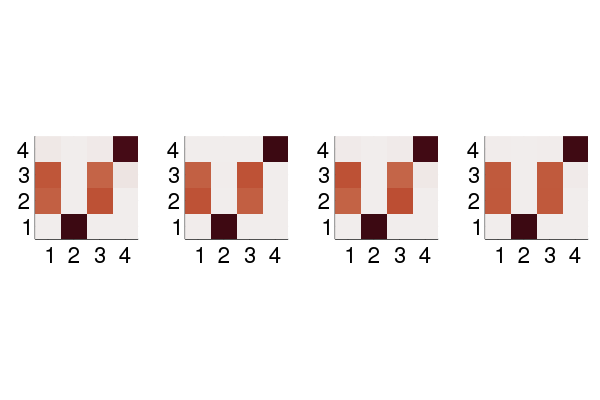
\includegraphics[width=0.40\linewidth,trim={2.0cm, .2cm, 2cm, 1.2cm}, clip]{swapmats}

% \fbox{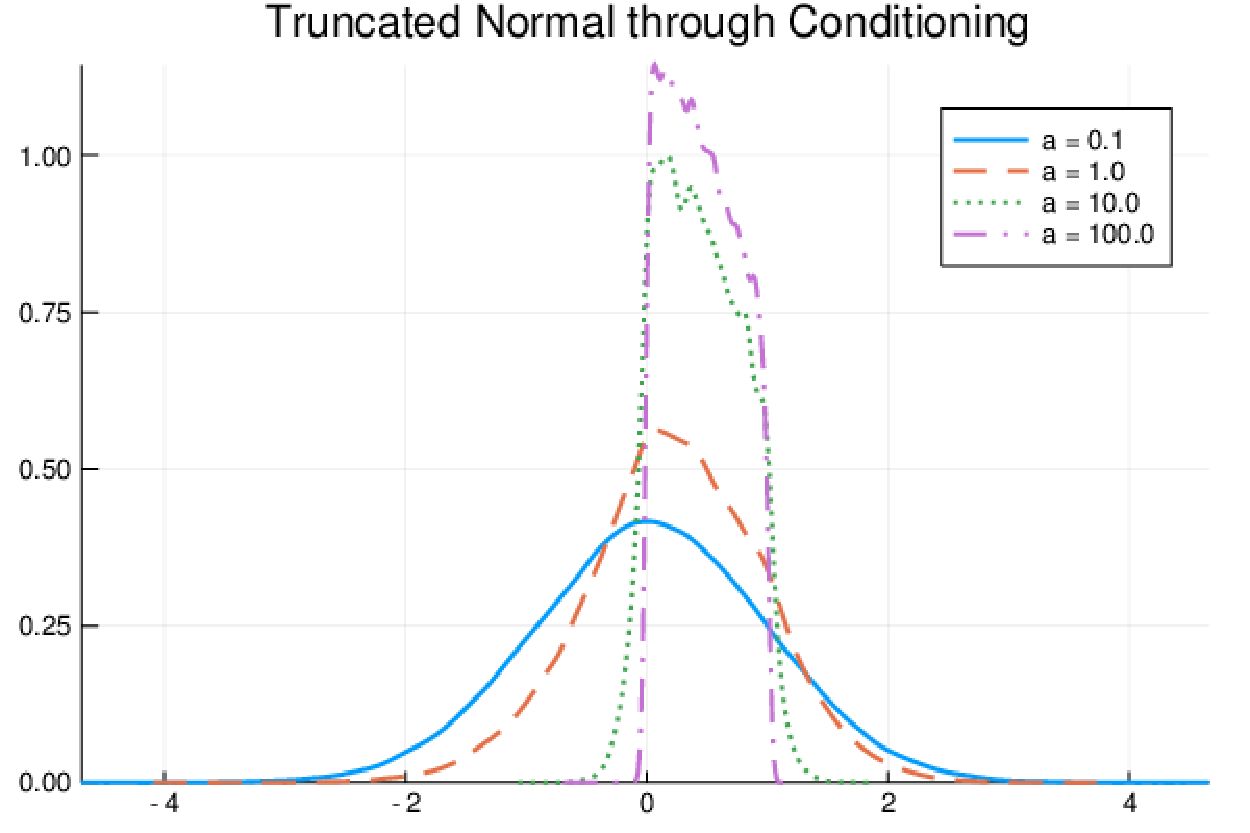
\includegraphics[width=1\linewidth,trim={0.5cm, .3cm, .5cm, .1cm}, clip]{truncated}}

% \begin{minipage}{0.45\linewidth}
% 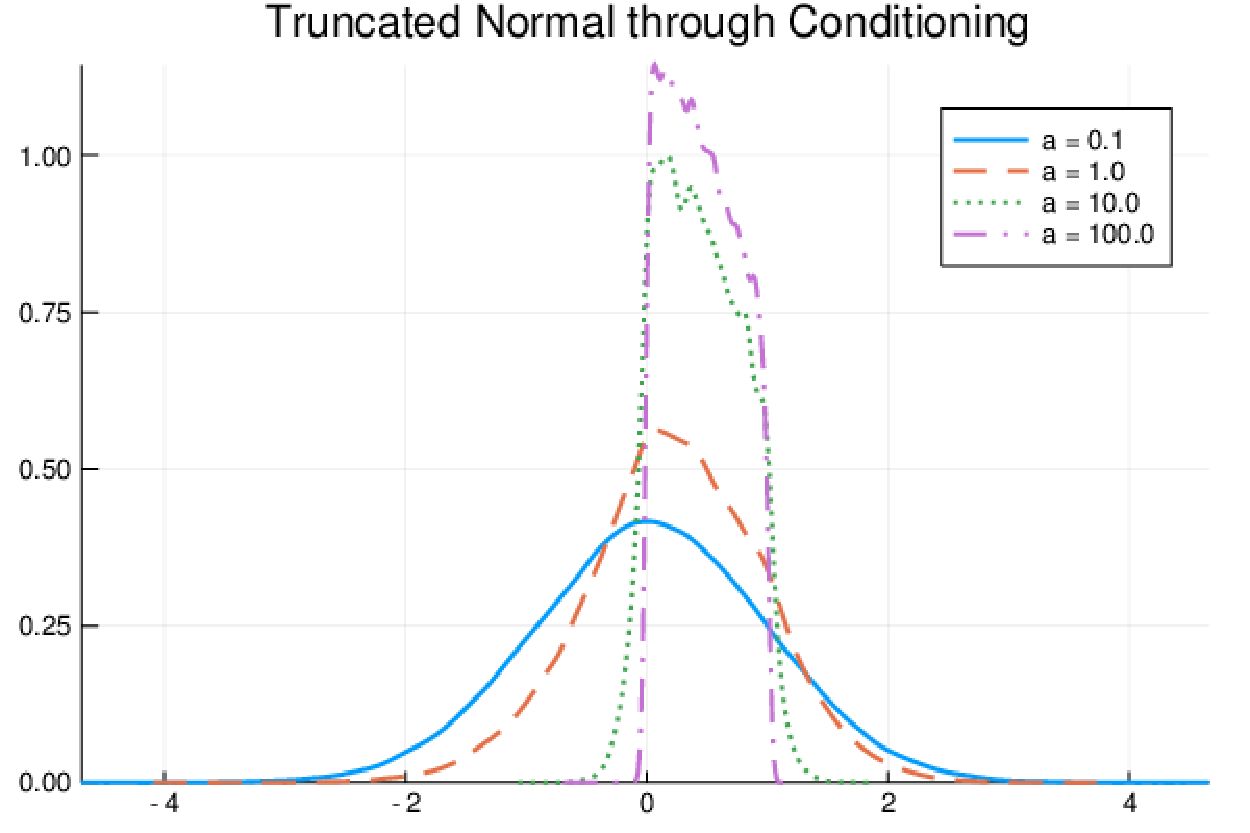
\includegraphics[width=\linewidth]{truncated}
% \end{minipage}%
% \begin{minipage}{0.45\linewidth}
% 	%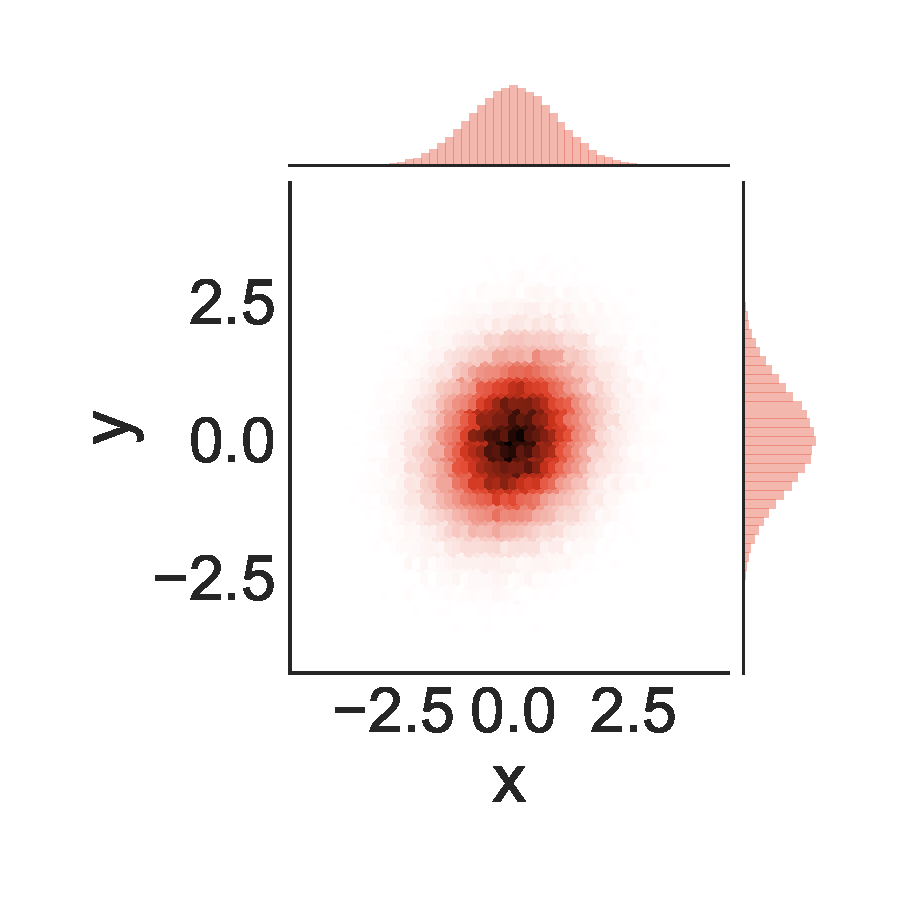
\includegraphics[width=.16\linewidth, trim={1.7cm, 1.6cm, 1.3cm, 1.5cm}, clip]{0-1}
% 	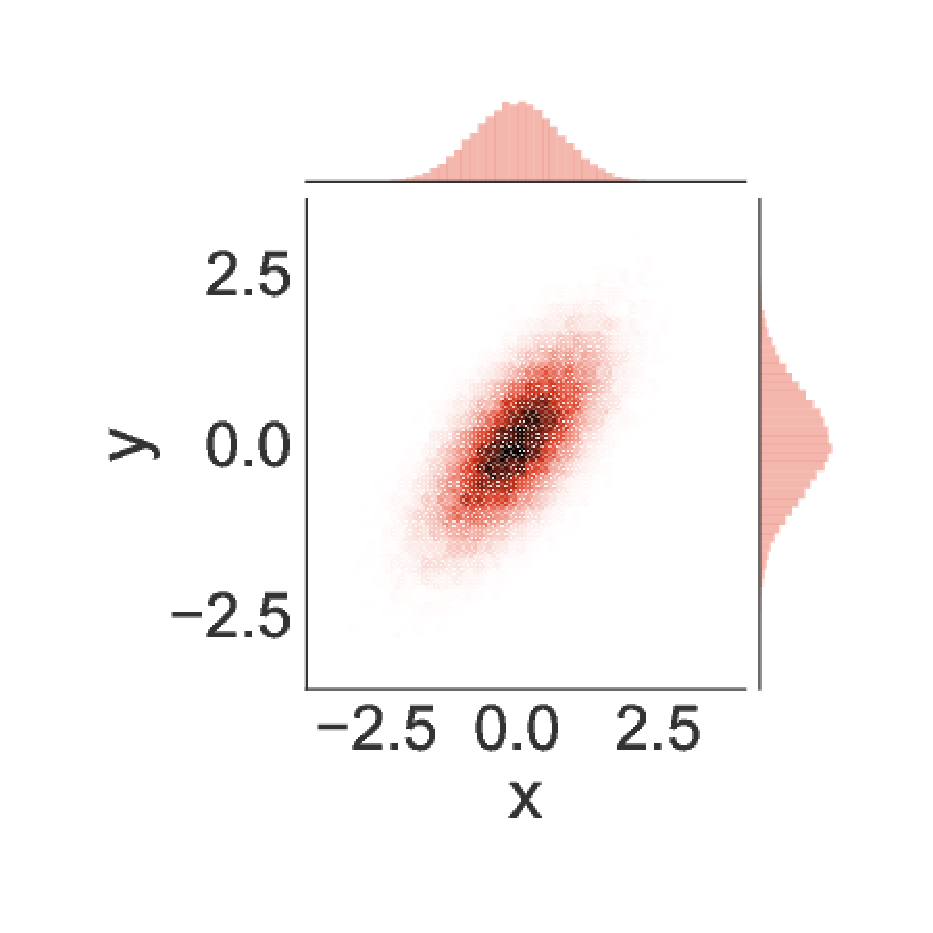
\includegraphics[width=.45\linewidth, trim={1.7cm, 1.6cm, 1.3cm, 1.5cm}, clip]{1-0}
% 	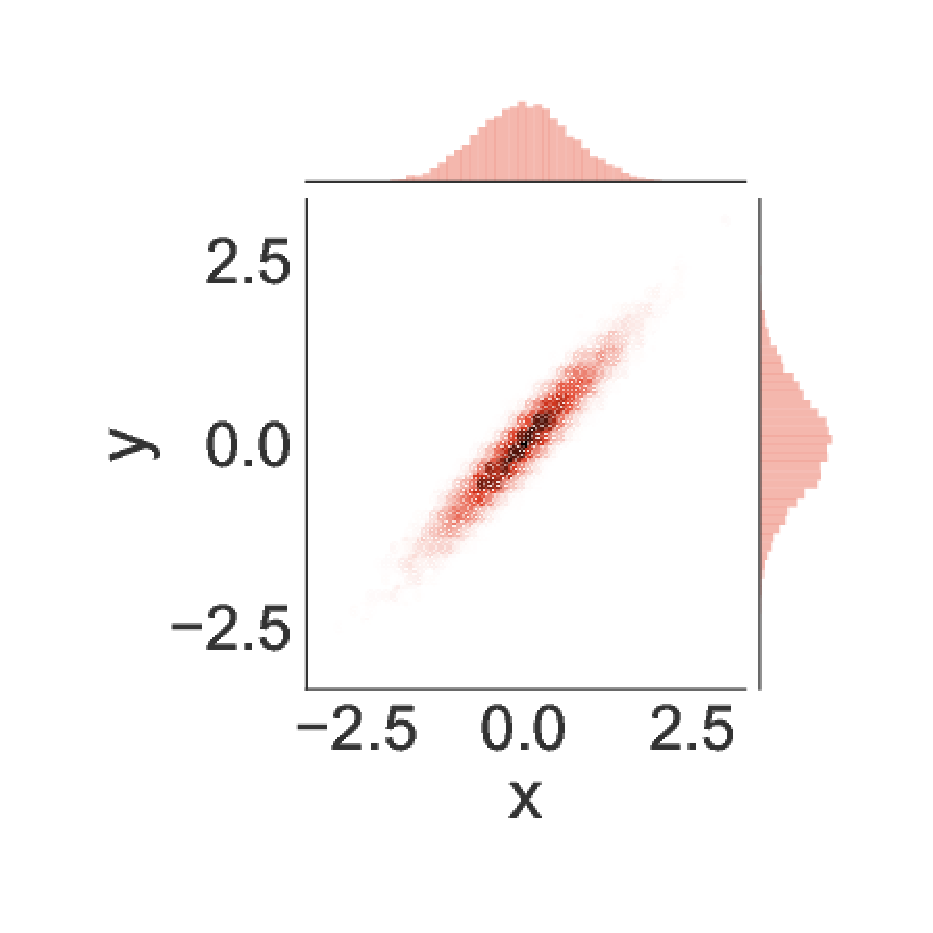
\includegraphics[width=.45\linewidth, trim={1.7cm, 1.6cm, 1.3cm, 1.5cm}, clip]{10-0}
	
% 	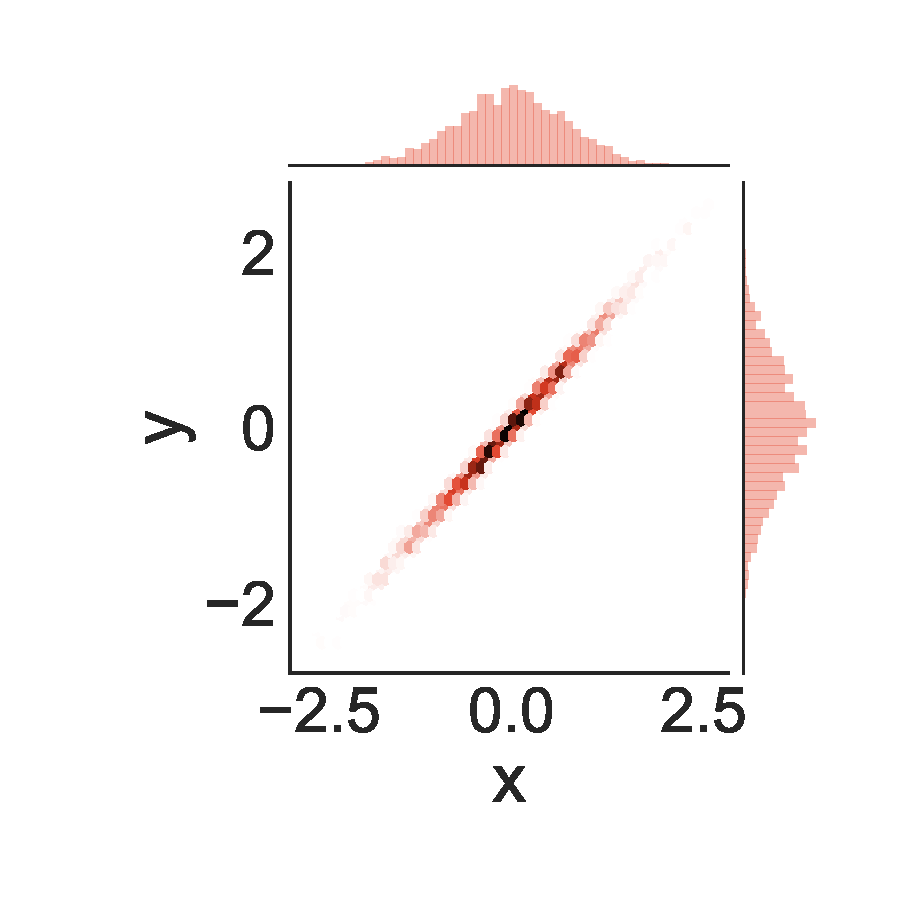
\includegraphics[width=.45\linewidth, trim={1.7cm, 1.6cm, 1.3cm, 1.5cm}, clip]{100-0}
% 	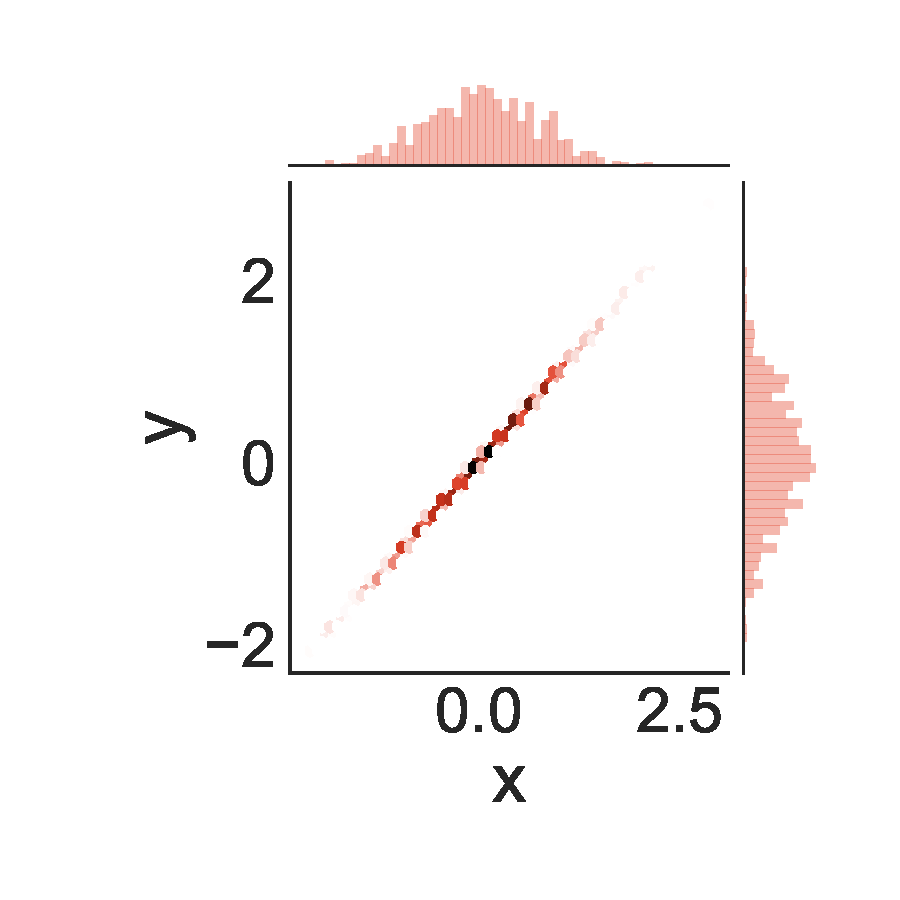
\includegraphics[width=.45\linewidth, trim={1.7cm, 1.6cm, 1.3cm, 1.5cm}, clip]{1000-0}				
	
% %	\fbox{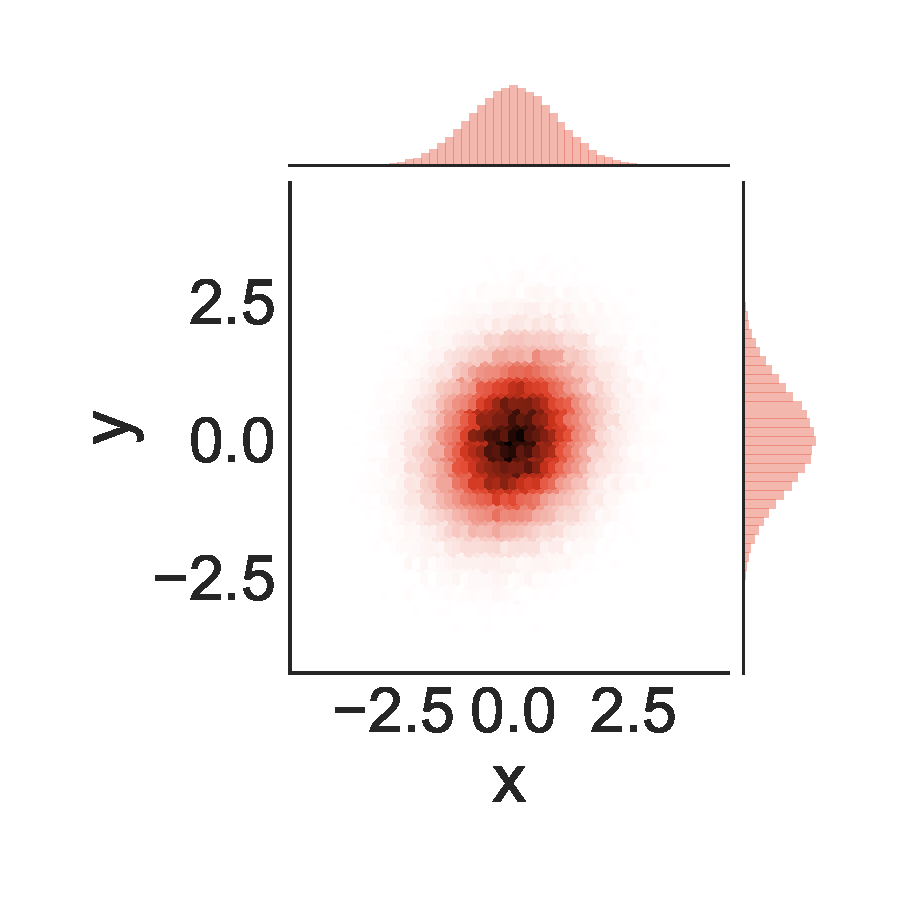
\includegraphics[width=.16\linewidth, trim={1.7cm, 1.6cm, 1.3cm, 1.5cm}, clip]{0-1}}
% %	\fbox{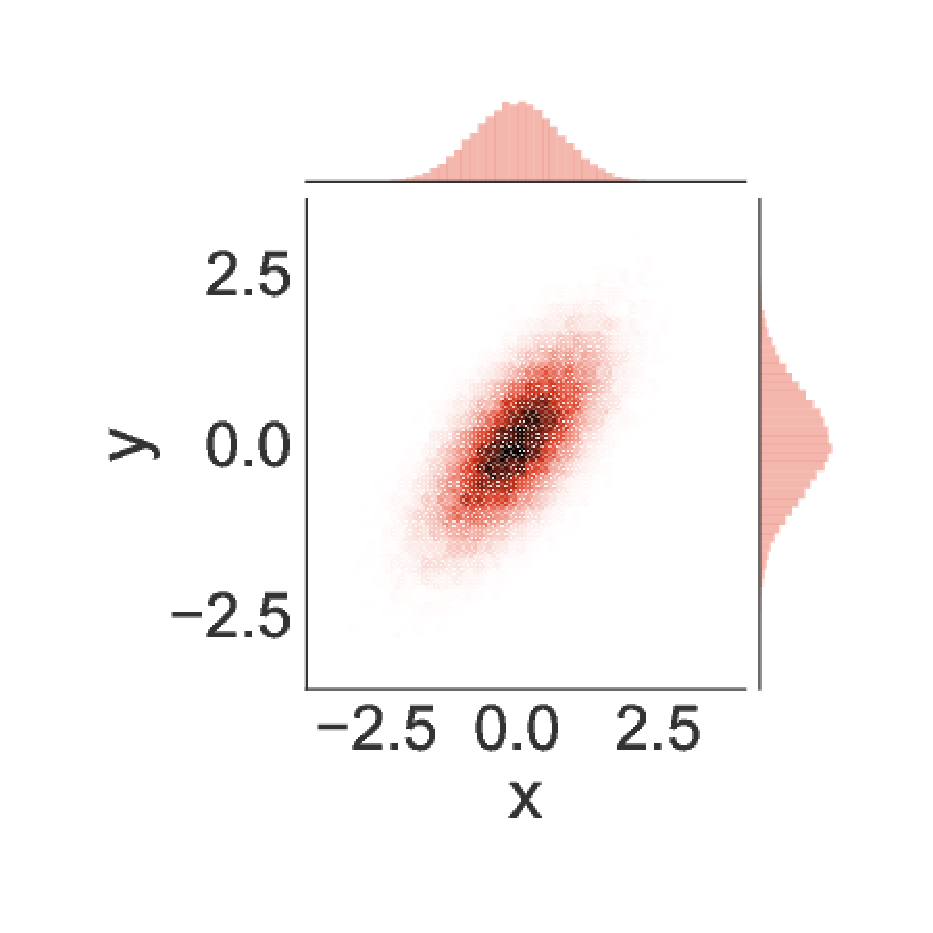
\includegraphics[width=.16\linewidth, trim={1.7cm, 1.6cm, 1.3cm, 1.5cm}, clip]{1-0}}
% %	\fbox{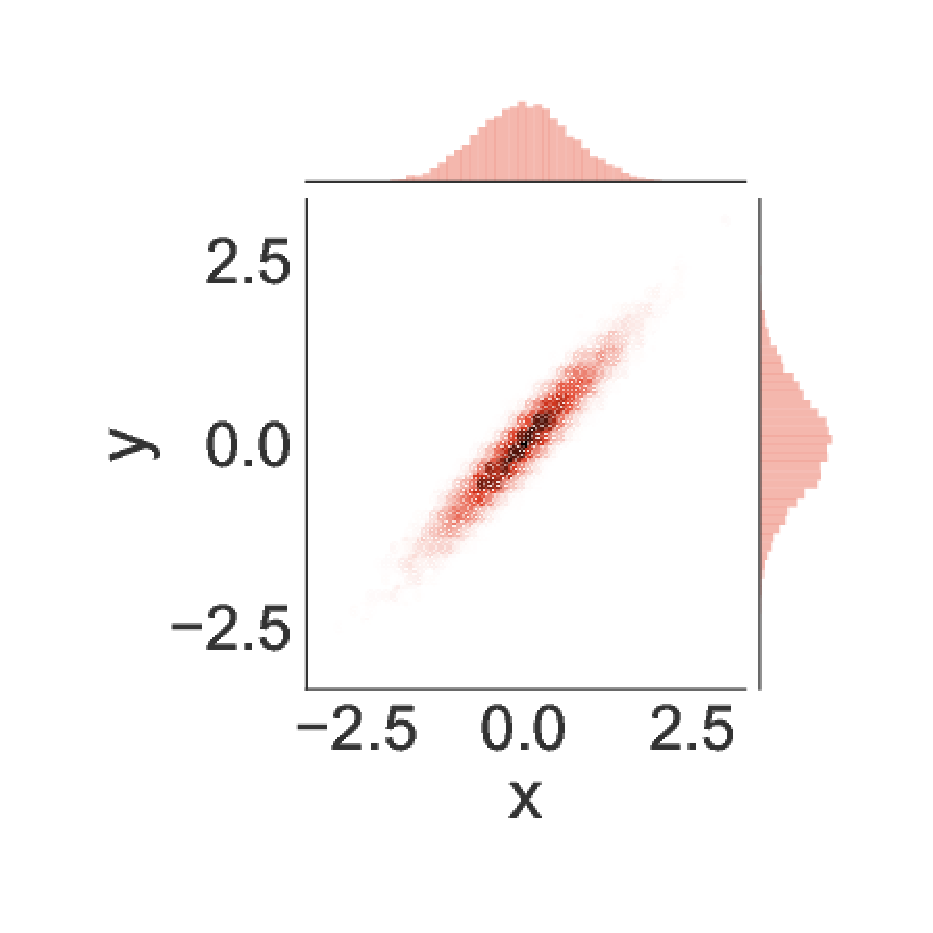
\includegraphics[width=.16\linewidth, trim={1.7cm, 1.6cm, 1.3cm, 1.5cm}, clip]{10-0}}
% %	\fbox{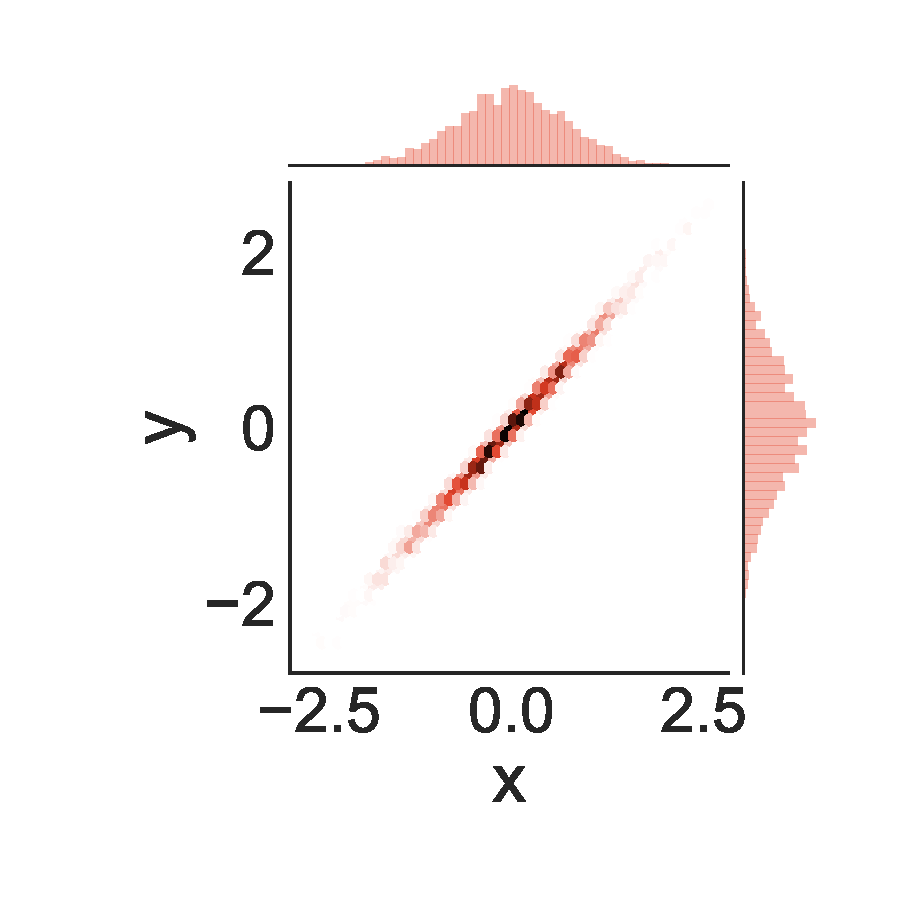
\includegraphics[width=.16\linewidth, trim={1.7cm, 1.6cm, 1.3cm, 1.5cm}, clip]{100-0}}
% %	\fbox{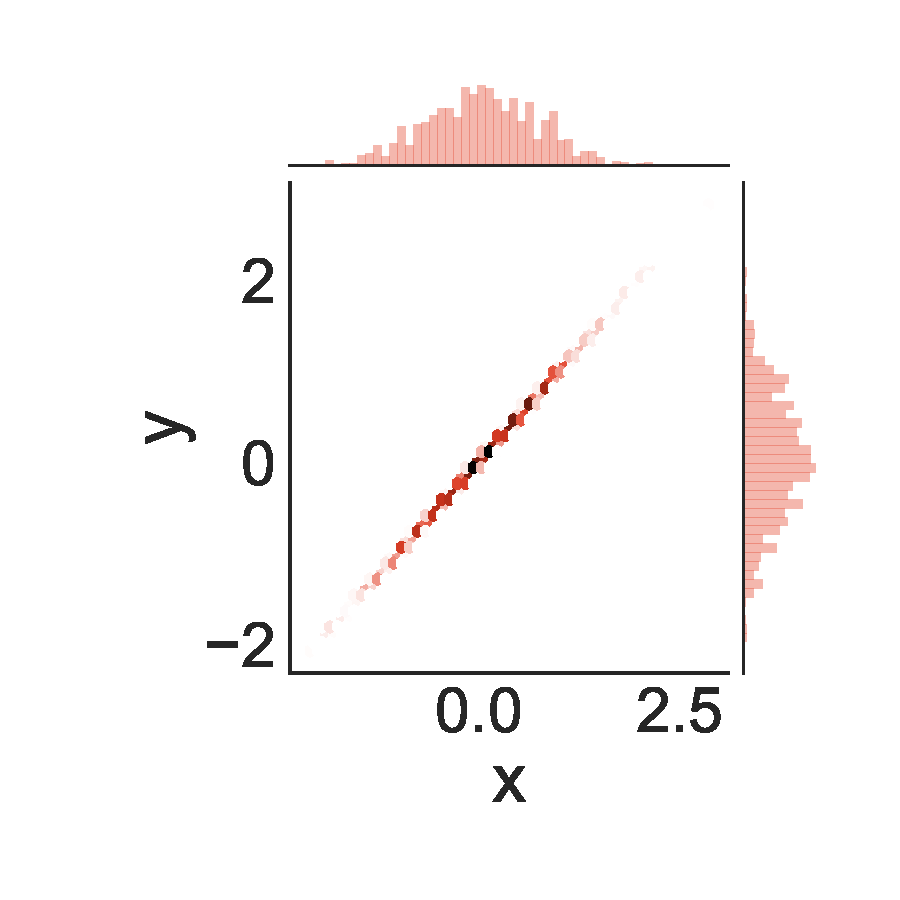
\includegraphics[width=.16\linewidth, trim={1.7cm, 1.6cm, 1.3cm, 1.5cm}, clip]{1000-0}}				
% 	\end{minipage}
	\caption{Kernel density estimation from samples of Gaussian truncated to $[0, 1]$ through conditioning. Shown at different temperatures.}
	\label{fig:density}
\end{figure}



\paragraph{Inverse Ray Tracing}
In this example we sample from a posterior distribution over scenes conditioned an observed rendering.  A scene $s$ is a set of $n \sim \textrm{poisson}(\lambda = 3)$ spheres.
A sphere is parameterized by color, reflectance, emission color, transparency, radius and position, all with a uniform prior.
Let $r$ be a ray tracing function that maps scenes to image, $i_{obs}$ be an observed image, and $\textrm{nointersect}$ be a predicate that maps a scene to 1 iff any spheres intersect.
The prior $s$ is conditioned on the conjunction of the inverse rendering and the no-intersection constraints:

\begin{equation}
(r(s) = i_{obs}) \land \textrm{nointersect}(s)
\end{equation}

Figure \ref{fig:invrtmcmc} visualizes conditional samples.
% \begin{figure}
% 	\centering
% 	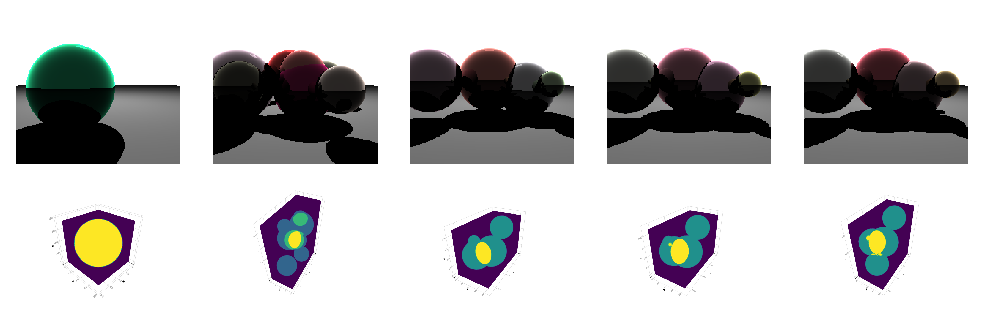
\includegraphics[width=0.9\linewidth]{invg2.pdf}
% 	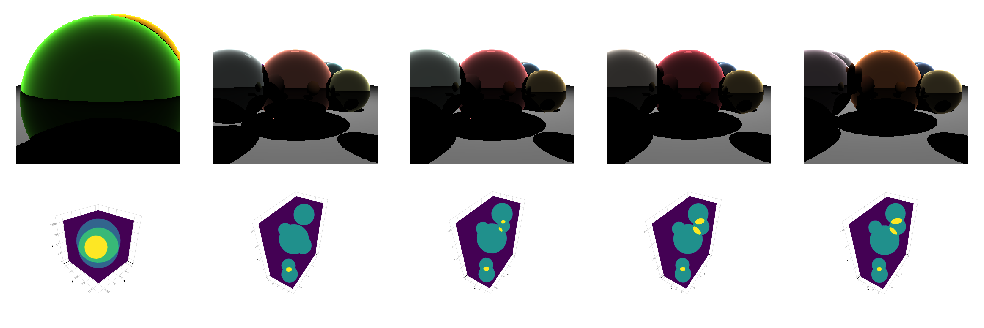
\includegraphics[width=0.9\linewidth]{invgb.pdf}
% 	% 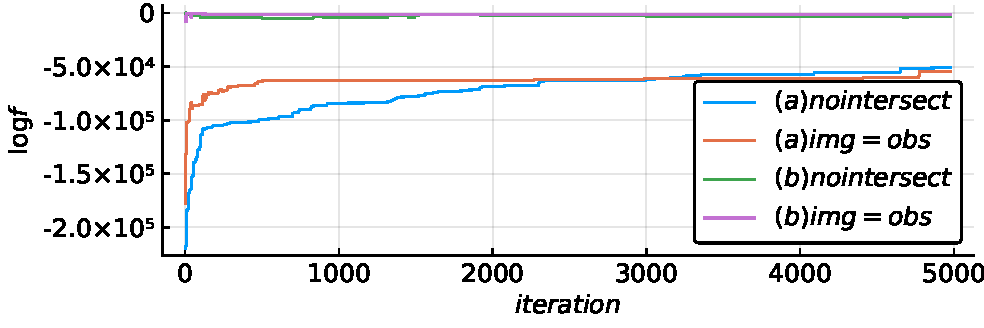
\includegraphics[width=0.9\linewidth]{lvstime.pdf}
% 	% 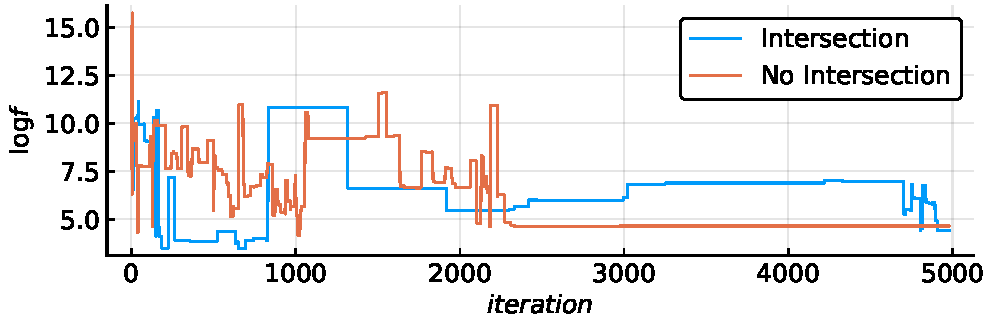
\includegraphics[width=0.9\linewidth]{Hausdorf.pdf}
% 	\caption{ Samples from inverse graphics.}
% 	\label{fig:invrtmcmc}
% \end{figure}

\begin{figure}
	\centering
	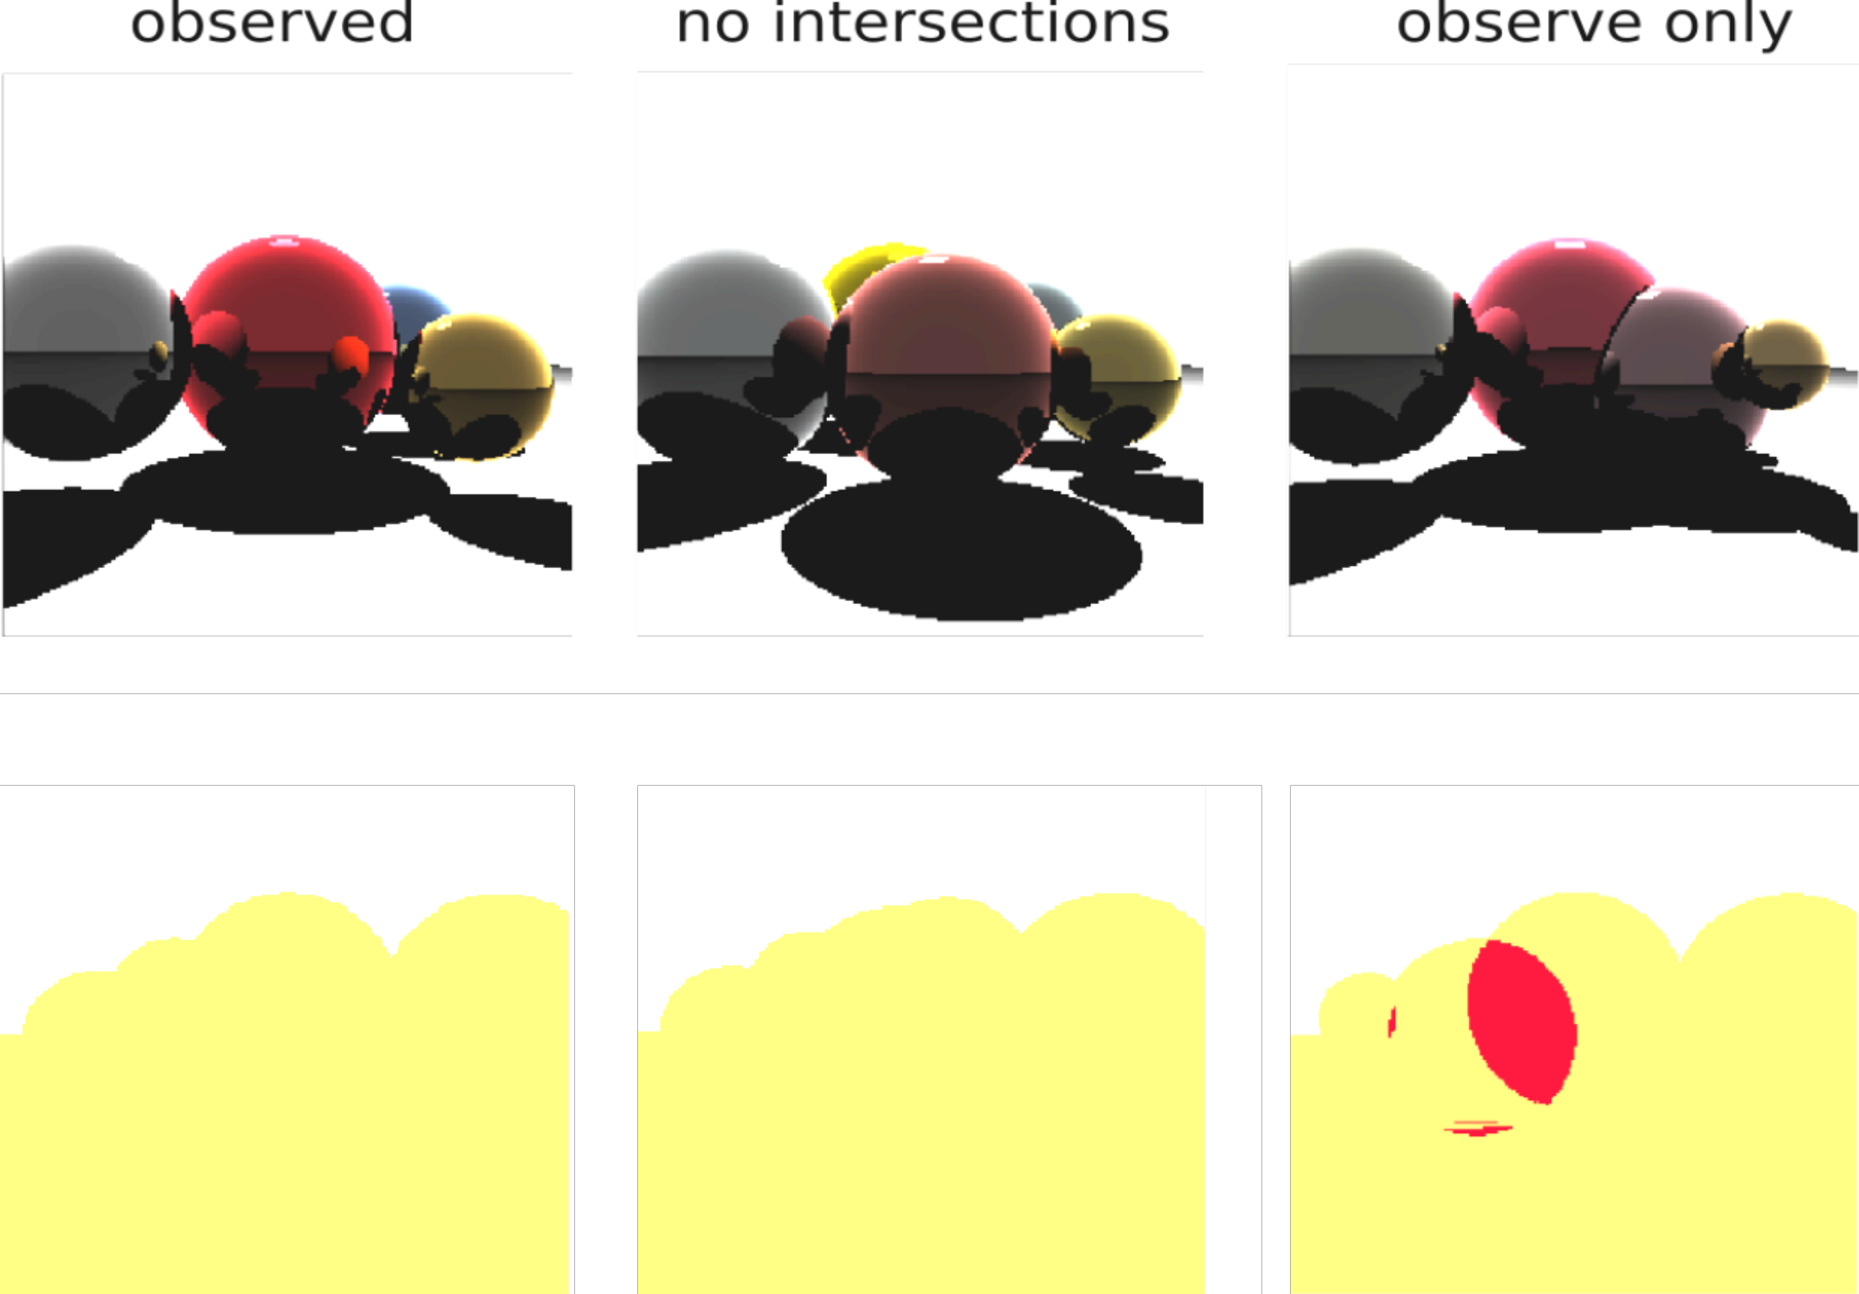
\includegraphics[width=0.9\linewidth]{jampy2.pdf}
	\caption{Inverse rendering with and without no-intersection constraints.  Top row: raytraced scenes.  Bottom row: red pixels denote the existence of an intersection between spheres at that point.  (middle) and (right) scenes are samples from posterior over scenes having observed image on left.  The observed scene has no intersections.  Without the no-intersection condition (right), intersections occur.  Conditioning on intersection eliminates intersections (middle).}
	\label{fig:invrtmcmc}
\end{figure}


\paragraph{Glucose Model}
Type 2 diabetes is a prevalent and costly condition.
Keeping blood glucose within normal limits helps prevent the
long-term complications of Type 2 diabetes like diabetic neuropathy and diabetic retinopathy \citep{brownlee2006glycemic}. Models to predict the trajectories of blood glucose aid in keeping glucose within
normal limits \citep{zeevi2015personalized}. Traditional models have been built from compositions of differential equations \citep{albers2017personalized,levine2017offline} whose parameters are estimated separately for each patient. An alternative approach would be to use a flexible sequence model like an RNN. The problem with this approach is that an RNN can extrapolate to glucose values incompatible with human physiology. This is especially a problem where we have patients with only a few blood glucose measurements. To build an RNN model that respects physiology, we condition on it.

We compare the independent RNN model to the one with declarative knowledge on a second patient from Physionet \citep{moody2001physionet}.
Figure \ref{fig:rnn-samples} plots the results performed on more than 300 pairs of patients.
We see that the conditional model simulates
more realistic glucose dynamics for the patient 
with only a short observed time-series.

% 1) Glucose modeling is a real problem \cite, \cite. 
% 2) Models have focused on ODEs \cite \cite 
% 3) Alternative is to use RNN 
% 4) RNN can produce nonsense result 
% 5) Conditioning helps


% Taken from the supplement in \cite{albers}

% \paragraph{A constrained model of glucose dynamic}
% Take glucose measurements across time $t$ from 
% N patients indexed by $i$: $x_{t,i}$.
% We model the glucose time series for each patient can be modeled independently using a recurrent neural network: 
% \begin{align*}
% W_i &\sim N(0, I) \\
% x_{t, i} &= f(x_{t-1, i}, W).
% \end{align*}
% This model treats all patients as independent. However,
% we have extra knowledge in that the average-across-time glucose levels will be similar across patients. Expressing this kind of knowledge by tying the parameters $W_i, W_j$ is a challenge because the structure of the recurrence function alters how $W$ controls the average outputs. In this sense, we would like to condition on the distance between conditional expectations being close for some distance $d$,
% \begin{align*}
% 	E\left(\sum_{t=1}^{T_i} E[x_{t, i} \,|\, W_i], \sum_{t=1}^{T_j} E[x_{t, j} \,|\, W_j]\right) < \delta_E,
% \end{align*}
% for all patient pairs $i, j$. Additionally, we would like to make the series smooth controlling for their variance:
% \begin{align*}
% 	d_{Var}\left(\sum_{t=1}^{T_i} Var[x_{t, i} \,|\, W_i], \sum_{t=1}^{T_j} Var[x_{t, j} \,|\, W_j]\right) < \delta_{Var},
% \end{align*}
%  We compare the independent model
% to the one with the conditional model learned on five patients. 
% We see that the conditional model simulates more realistic glucose dynamics for the patient with only a short observed time-series.

\begin{figure}[!htb]
	\centering
    %\fbox{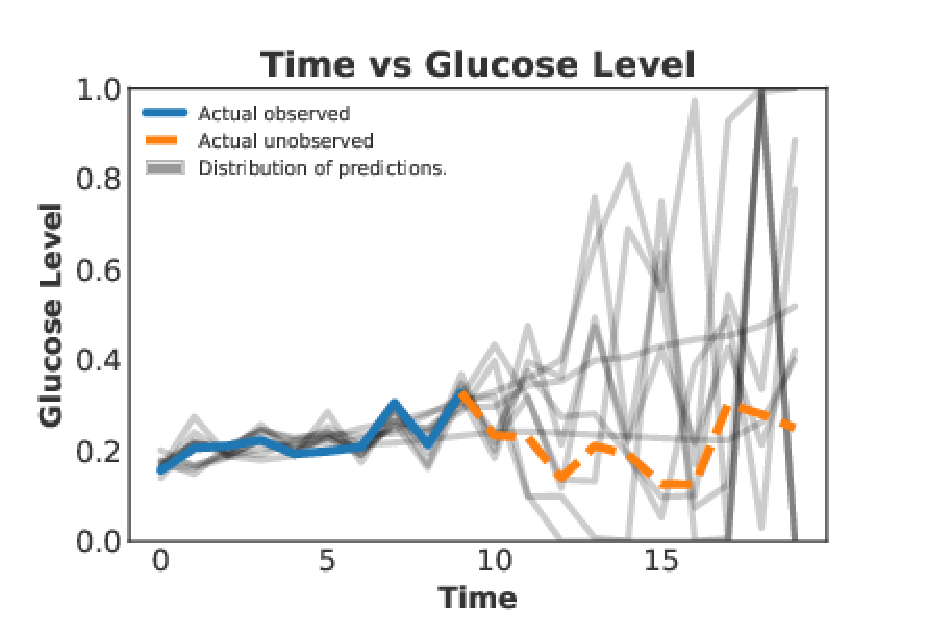
\includegraphics[width=0.30\linewidth, trim={1.cm, 0.1cm, 1.3cm, .5cm}, clip]{rnnsamples-no-tie-py}}
	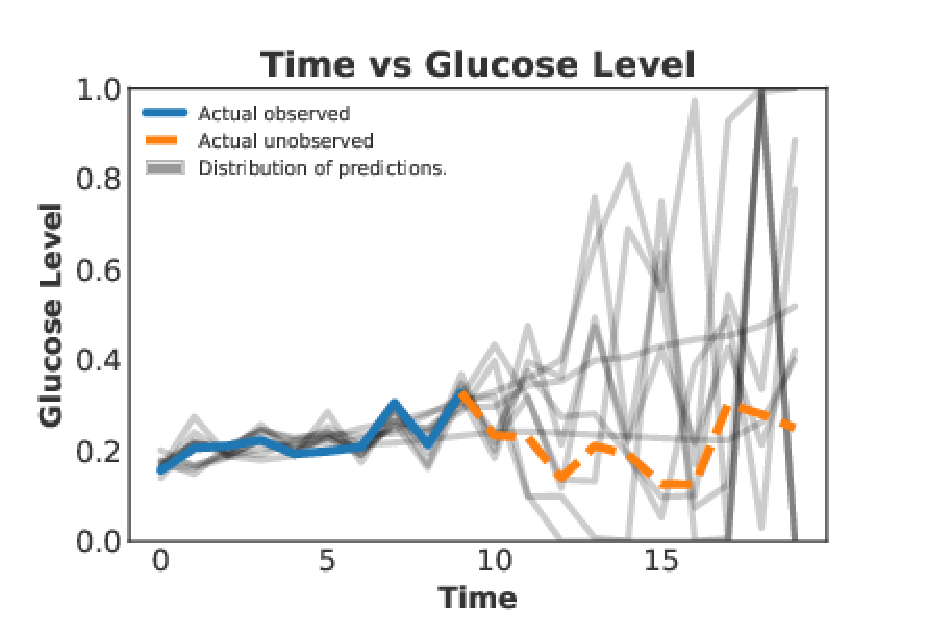
\includegraphics[width=0.8\linewidth, trim={1.cm, 0.1cm, 1.3cm, .5cm}, clip]{rnnsamples-no-tie-py}
	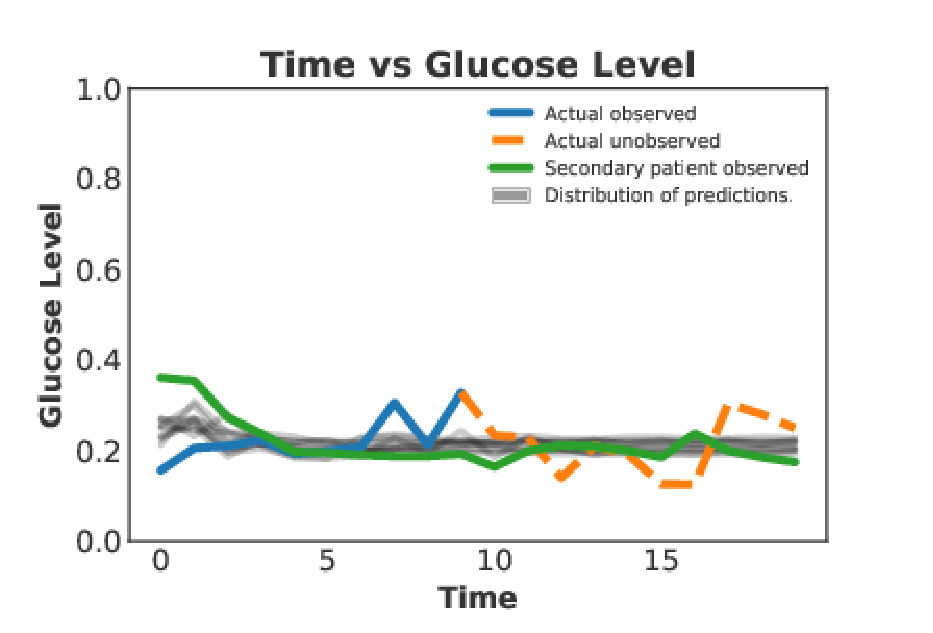
\includegraphics[width=0.8\linewidth, trim={1.cm, 0.1cm, 1.3cm, .5cm}, clip]{rnnsamples-py}
	%\fbox{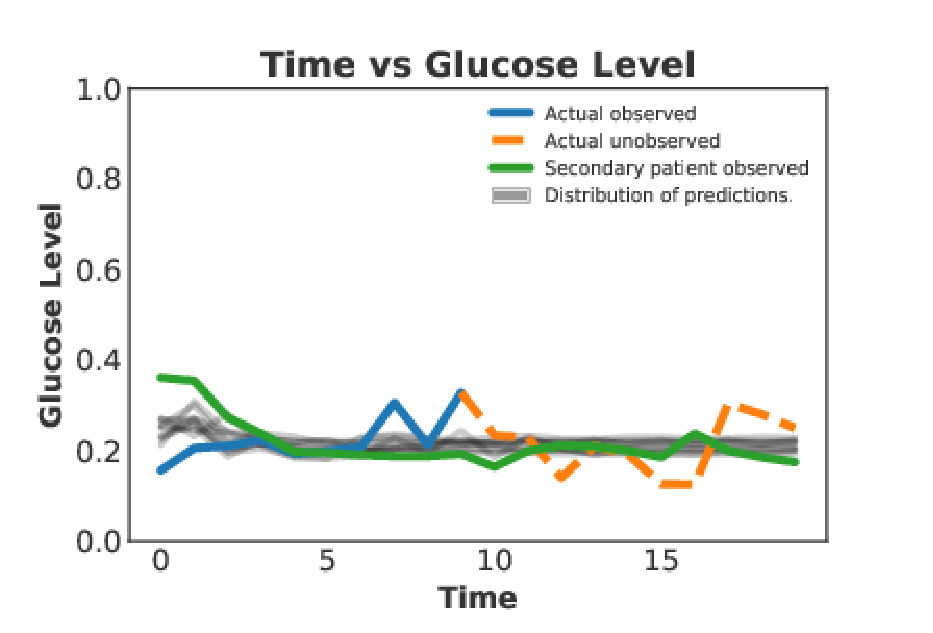
\includegraphics[width=0.30\linewidth, trim={1.cm, 0.1cm, 1.3cm, .5cm}, clip]{rnnsamples-py}}
	%\fbox{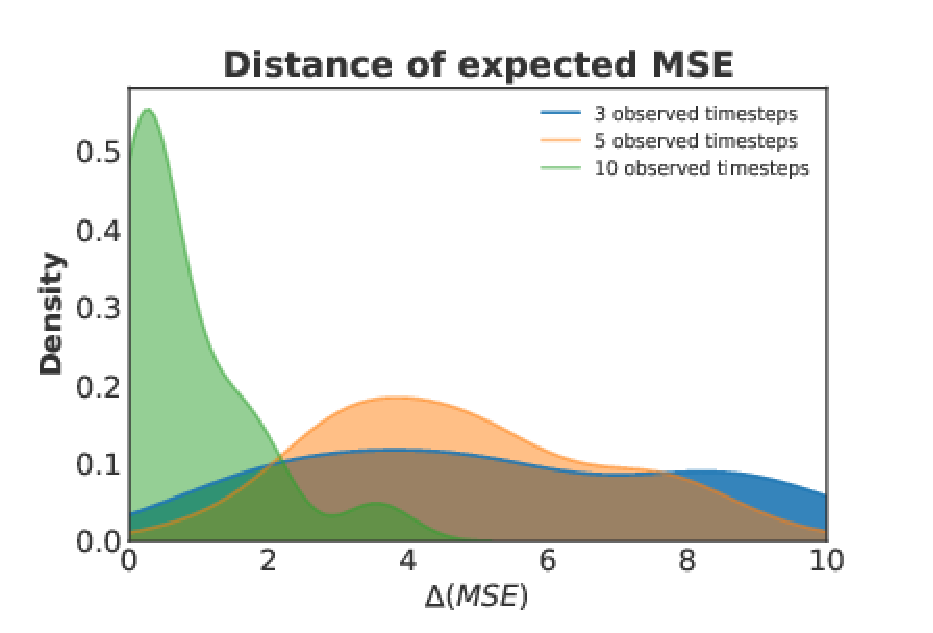
\includegraphics[width=0.30\linewidth, trim={1.cm, 0.0cm, 1.0cm, .5cm}, clip]{delta_mse}}
	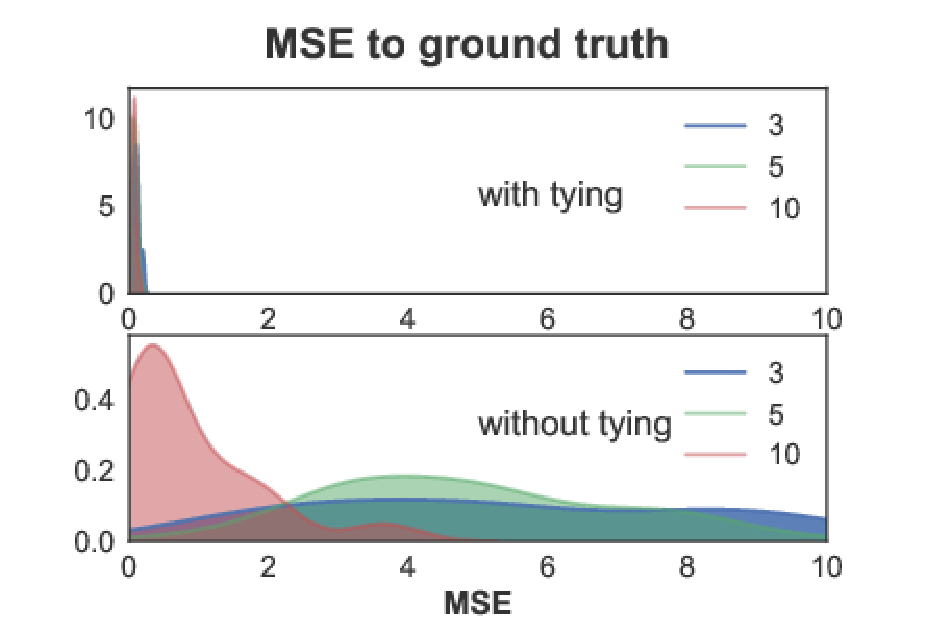
\includegraphics[width=0.9\linewidth, trim={0.7cm, 0.0cm, .7cm, .1cm}, clip]{mse}
		
		\caption{Left: Actual (dotted) and predicted trajectories that were learned using a partial trajectory. Center: Distribution of predicted trajectories learned only using the first ten data points and a tie with a secondary patient. Right, top: MSE when tie is present.  Right, bottom: without tie.  Tying expectations has dramatic influence on prediction error, while as more data is observed, the effect of tying decreases.}
		\label{fig:rnn-samples}
\end{figure}



% Take the same glucose measurements from 5 patients. Make a probabilistic RNN with
% independent parameters for each patient. Then add the constraint that the means are
% close. Then look at the prediction for one patient where we remove all but the
% first few time steps and show the forward predictions are better with the added knowledge
% that the means are close across patients.


% \paragraph{Transfer Learning}
% In transfer learning, we hope to use information from one learning problem to
% help with another learning problem. One way this has been accomplished in
% deep learning is to use
% the parameters of a model learned in one domain as the initialization for the
% parameters in a another domain. We could accomplish a similar thing via conditioning
% by having the weights of both models be close. But with conditioning, this is not
% the only choice, we can have the first layer activations be close in distribution
% in both the source and target transfer domain. Concretely, consider the following
% two layer stochastic neural network for each domain where the $i$th covariate
% label pair $(x_i, y_i)$ is
% \begin{align*}
% W \sim p(W)
% z_{2, i} &\sim p(z_{2, i} | x_i, W_2) \\
% z_{1, i} &\sim p(z_{1, i} | z_{2, i}, W_1) \\
% y_{i} &\sim p(y_i | z_{1, i})
% \end{align*}


% \section{Related Work}
% \begin{itemize}

% \item Existing Notion of Probablistic Programs
% Probabilistic programming languages and the inference algorithms which support them differ primarily in how probability distributions are represented.
% % In this contribution we define the sample space as an $n$-dimensional unit hypercube
% % $\Omega = [0, 1]^n$, and by $(\omega_1,...,\omega_n)$ denote an element of $\Omega$.
% % In addition, we define $\mu$ as the Lebesgue measure.
% % Random variables are transformations of $\Omega$, and act on some or all of its dimensions.
% % For example a random variable $\mathcal{U}_{a,b}: \Omega \to \mathbb{R}$, which is distributed uniformly between $a$ and $b$ could be defined simply as:
% % $$
% % \mathcal{U}_{a,b}(\omega) = a + \omega_1(b - a)
% % $$
% \item Make explicit how the measure theortic formulation connects to the sampling process
% \end{itemize}


\paragraph{Benchmarks}
To quantitatively compare predicate exchange with existing approaches we constructed an artificial problem that scales in difficulty.
Let $X_i \sim \mathcal{N}(0,1)$ in a $d$-dimensional model $\vect{X} = (X_1, \dots, X_d)$ conditioned on an $\epsilon$-thick ring:
\begin{equation}
\lk_\epsilon(\vect{x}) = 1 < |\vect{x}| < 1 + \epsilon
\end{equation}

Table \ref{results} compares the sample average of particle Gibbs (PG), sequential Monte Carlo (SMC), rejection sampling (RS) and predicate exchange (PE), varying both $\epsilon$ and $d$.
The theoretical expectation of all models is 0.
Among these methods, predicate exchange is unique in its support for inference with predicates, which makes direct comparison difficult.
For all inference procedures we use predicate relaxation to compute $d = \softv{\lk}_\epsilon(\vect{x})$, and sample from $\vect{X}$ conditioned on $\mathcal{N}(d, 1/(2\alpha)) = 1$, where $\alpha$ is the lowest temperature used in predicate exchange.
Predicate exchange  compares favourably in most scenarios.


\begin{figure}
\begin{center}
	\begin{tabular}{||c| c c c c||} 
	\hline
	 $d,\epsilon$& $1, {10^{-1}}$ & $1, {10^{-5}}$ & ${100}, {10^{-1}}$ & ${100}, {10^{-5}}$ \\ [0.5ex] 
	\hline\hline
	PE & 0.0054 & 0.4735  & -0.00037 & 0.00854\\ 
	\hline
	% HMC & 2.1 & 2.026  & 1.5 & 1.41\\ 
	% \hline\hline
	SMC & 0.06 & -0.226  & -0.018 & 0.09\\ 
	\hline
	PG & -0.029 & 0.239 & -0.03 & 0.03\\
	\hline
	RS & 0.003 & timeout & timeout & timeout \\
	\hline
 \end{tabular}
 \label{results}
 \caption{Comparison of expectations of samples from $d$ dimensional ring.  Theoretical value is 0 in all cases.}
 \end{center}
\end{figure}


  